\section{První týden}

\subsection{Důkaz souvislosti minima a maxima}

Tvrzení. Pro $f: D \rightarrow \R, M \subseteq D, \hat{x} \in M$ platí:

\begin{enumerate}[(1)]
    \item $\hat{x} \in \underset{x \in M}{\argmin} f(x) \iff \hat{x} \in \underset{x \in M}{\argmax} (-f(x))$,
    \item jesliže $\hat{x} \in \underset{x \in M}{\argmin} f(x)$, pak $\underset{x \in M}{\min} f(x) = 
    - \underset{x \in M}{\max} (-f(x))$.
\end{enumerate}
Důkaz.

(1) $\hat{x} \in \underset{x \in M}{\argmin} f(x)$, tj. $f(\hat{x}) \leq f(x), \forall x \in M \underset{\cdot (-1)}{\iff} 
-f(\hat{x}) \geq -f(x), \forall x \in M$, tj. $\hat{x} \in \underset{x \in M}{\argmax} (-f(x)). \qed$


(2) Ať $\hat{x} \in \underset{x \in M}{\argmin} f(x)$, pak $\underset{x \in M}{\min} f(x) = f(\hat{x}) = 
- (- f(\hat{x})) \overset{(1)}{=} - \underset{x \in M}{\max} (-f(x)). \qed$

\subsection{Hledání přípustných množin}
\begin{align*}
    \text{minimalizujte } x^2 + 1 \\
    \text{za podmínek } \frac{3}{x} \leq 1, \\
    x \in \N.
\end{align*}
Upravíme podmínky a uděláme jejich průnik: $(x - 3 \geq 0) \land (x \in \N) \Rightarrow M = \N \setminus \bc{1,2}$.

Úvahou pak lze uhodnout minimum - minimum leží v bodě $x=3$.

\subsection{Hledání přípustných množin}
\begin{align*}
    \text{maximalizujte } \ln x \\
    \text{za podmínek } x \leq 5, \\
    \cos(\pi x) = 1.
\end{align*}
$D(f) = (0, \infty)$. 

Udělejme průnik definičního oboru funkce a podmínek: $(x \in (0, \infty)) \land (x \leq 5) \land (\cos(\pi x)=1)$.

\begin{multicols}{2}
    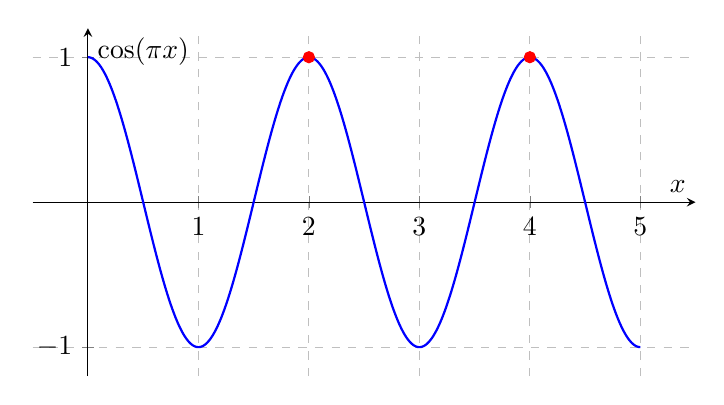
\begin{tikzpicture}
        \begin{axis}[
            axis lines = middle,
            xlabel = $x$,
            ylabel = {$\cos(\pi x)$},
            domain=0:5,
            samples=1000,
            %   xtick={0,1,2,3,4,5},
            %   ytick={-1,-0.5,0,0.5,1},
            enlargelimits,
            grid=both,
            minor grid style={dotted},
            major grid style={dashed},
            width=10cm, height=6cm,
        ]
            \addplot[blue, thick] {cos(deg(x * pi))};
            \addplot[only marks, red, mark=*] coordinates {(2,1) (4,1)};
        \end{axis}
      \end{tikzpicture}
\columnbreak

      \quad Očividně tedy $M = \bc{2,4}$.

      \quad Úvahou pak lze uhodnout $\underset{x \in M}{\argmax} \ln x = \bc{4}$.
\end{multicols}

\subsection{Uzavřená úsečka}
Nechť $x, y \in \R^n$. Množina
\[ [x,y] := \bc{\lambda x + (1-\lambda)y \mid 0 \leq \lambda \leq 1} \]
se nazývá uzavřená úsečka s krajními body $x$ a $y$.

\subsection{Je nadrovina konvexní?}
Definice nadroviny: $H(y; \alpha) := \bc{x \in \R^n \mid \langle x, y \rangle = \alpha}$, $y \in \R^n$, $\alpha \in \R$.

Důkaz.

Ať $x,z \in H(y, \alpha), \lambda \in [0,1]$.\\
Cíl: $\lambda x + (1-\lambda) z \in H(y, \alpha)$. Tedy chceme dokázat, že úsečka mezi dvěma libovolnými body z množiny
také leží v množině. 

$\langle \lambda x + (1-\lambda)z, y \rangle = \lambda \underbrace{\langle x,y \rangle}_{\alpha} + (1-\lambda) 
\underbrace{\langle z,y \rangle}_{\alpha} = \lambda \alpha + (1-\lambda) \alpha = \alpha$.

$\Rightarrow \lambda x + (1-\lambda)z \in H(y, \alpha). \qed$

\subsection{Je uzavřený poloprostor konvexní?}

\subsection{Je uzavřená koule konvexní?}
Definice uzavřené koule: $B(a,r) = \bc{a \in \R^n \mid ||x -a || \leq r}$, o středu $a \in \R^n$ a poloměru $r > 0$. 

Důkaz.

Ať $x,y \in \R^n, \lambda \in [0,1]$.\\
Cíl: $|| [\lambda x + (1-\alpha)y] - a || \leq r$. Tedy za $x$ z definice dosadíme úsečku mezi body $x$ a $y$, které jsme
si vybrali a chceme ukázat, že i tato úsečka leží v uzavřené kouli.

\[
    || [\lambda x + (1-\alpha)y] - a || = || \lambda x - (1-\lambda)a + (1-\lambda)y - \lambda a || = 
    || \lambda (x-a) + (1-\lambda)(y-a) || 
\]
\[ 
    \leq \lambda ||\underbrace{x-a}_{\leq r}|| +  (1-\lambda)||\underbrace{y-a}_{\leq r}|| \leq \lambda r + (1-\lambda)r
     = r. \qed
\]

\subsection{Je okolí konvexní?}
Definice okolí: $B(a,r) = \bc{a \in \R^n \mid ||x -a || < r}$, o středu $a \in \R^n$ a poloměru $r > 0$. 

Důkaz.

Ať $x,y \in \R^n, \lambda \in [0,1]$.\\
Cíl: $|| [\lambda x + (1-\alpha)y] - a || < r$. Tedy za $x$ z definice dosadíme úsečku mezi body $x$ a $y$, které jsme
si vybrali a chceme ukázat, že i tato úsečka leží v okolí.

\[
    || [\lambda x + (1-\alpha)y] - a || = || \lambda x - (1-\lambda)a + (1-\lambda)y - \lambda a || = 
    || \lambda (x-a) + (1-\lambda)(y-a) || 
\]
\[ 
    \leq \lambda ||\underbrace{x-a}_{< r}|| +  (1-\lambda)||\underbrace{y-a}_{< r}|| < \lambda r + (1-\lambda)r
     = r. \qed
\]

\subsection{Je průnik množin konvexní?}
Nechť $x,y \in \bigcap\limits_{i \in I} \mathbb{M}_{i}, \forall i \in I \implies [x, y] \in \mathbb{M}_i, \forall i \in I
\implies [x,y] \subseteq \bigcap\limits_{i \in I} \mathbb{M}_{i}. \qed$

\subsection{Důkaz, že rozdíl a sjednocení nezachovává konvexitu}
% Mějme $\underbrace{[0,1]}_{\text{přímka}} \setminus \underbrace{(0,1)}_{\shortstack{\text{\scriptsize otevřený} \\ \text{\scriptsize interval}}} = \bc{0,1} = \bc{0} \cup \bc{1}$.
Mějme $[0,1] \setminus (0,1) = \bc{0,1} = \bc{0} \cup \bc{1}$.

$[0,1]$ a $(0,1)$ jsou konvexní množiny. Jejich rozdíl ale už konvexní není.\\
$\bc{0}$ a $\bc{1}$ jsou konvexní množiny. Jejich sjednocení ale už konvexní není.

\subsection{Důkaz, že afinní zobrazení je konvexní}
Tvrzení. $f: \R^n \rightarrow \R^m$, $f$ je afinní $\iff$ pro každé $x,y \in \R^n$ a každé $\lambda \in \R$ je
\[f(\lambda x + (1-\lambda) y) =\lambda f(x) + (1-\lambda) f(y)\text{.}\]

Důkaz.

"$\Rightarrow$": Ať $f(x) = Ax + b$, kde $A \in \mathbb{M}_{m,n} (\R)$, $b \in \R^n$.

Ať $x, y \in \R^n, \lambda \in \R$.
\[
    f(\lambda x + (1 - \lambda) y) = A [\lambda x + (1-\lambda) y] + b = \lambda A x + (1-\lambda)Ay + \lambda b + 
    (1-\lambda)b = 
\] 
\[ 
    \lambda \underbrace{(Ax + b)}_{f(x)} + (1-\lambda)\underbrace{(Ay + b)}_{f(y)} = \lambda f(x) + (1-\lambda)f(y). \qed
\]

"$\Leftarrow$": Ať $\varphi(x) = f(x) - f(0)$.\\
Cíl: $\varphi$ je lineární zobrazení.

Musíme ověřit uzavřenost na násobení a sčítání.

(1) Ať $x \in \R^n$, $\alpha \in R$.\\
Cíl: $\varphi(\alpha x) = \alpha \varphi(x)$.
\[
    \varphi(\alpha x) = f(\alpha x) - f(0) = f(\alpha x + (1-\alpha)0) - f(0) = \alpha f(x) + (1-\alpha)f(0) - f(0) =
\]
\[
    \alpha f(x) - \alpha f(0) = \alpha (f(x) - f(0)) = \alpha \varphi (x-0). \qed
\]

(2) Ať $x, y \in \R^n$.\\
Cíl: $\varphi(x+y) = \varphi(x) + \varphi(y)$.
\[
    \varphi(x+y) = \varphi \left(2 \left(\frac{1}{2} (x+y)\right)\right) \stackrel{(1)}{=} 2 \varphi \left(\frac{1}{2} (x+y)\right) = 
    2 \left[f(\frac{1}{2}x + \frac{1}{2}y) - f(0)\right] = 2 \left[\frac{1}{2} f(x) + \frac{1}{2}f(y) - f(0) \right] = 
\]
\[
    f(x) + f(y) - f(0) - f(0) = \underbrace{f(x) - f(0)}_{\varphi(x)} + \underbrace{f(y) - f(0)}_{\varphi(y)} = 
    \varphi(x) + \varphi(y). \qed
\]

\subsection{Důkaz, že obraz konvexní množiny při afinním zobrazení je konvexní}
Tvrzení. 

Je-li $f: \R^n \rightarrow \R^m$ afinní a $C \subseteq \R^n$ konvexní, pak $f(C)$ je konvexní.

Důkaz.

Mějme $a, b \in f(C) \implies \exists x, y \in C: f(x)=a, f(y)=b$.

Dle předpokladu je $C$ konvexní. $\implies [x, y] \subseteq C \implies \underbrace{f([x, y])}_{\subseteq f(C)} = 
[\underbrace{f(x)}_a, \underbrace{f(y)}_b] \subseteq f(C). \qed$

\newpage
\subsection{Důkaz, že kartézský součin je konvexní}
Tvrzení.

Nechť $C_1 \subseteq \R^n$ a $C_2 \subseteq \R^m$. Pak $C_1$ a $C_2$ jsou konvexní množiny právě tehdy, když 
$C_1 \bigtimes C_2$ je konvexní množina.

Důkaz.

"$\Rightarrow$": Mějme 
$
\begin{bmatrix}
    a \\
    b
\end{bmatrix}\hspace{-1mm}\text{,}
\begin{bmatrix}
    c \\
    d
\end{bmatrix} \in C_1 \bigtimes C_2, \lambda \in [0,1]$\\
Cíl: 
$
\lambda \begin{bmatrix}
    a \\
    b
\end{bmatrix}
+ (1-\lambda)
\begin{bmatrix}
    c \\
    d
\end{bmatrix} \in C_1 \bigtimes C_2.$

$
\lambda \begin{bmatrix}
    a \\
    b
\end{bmatrix}
+ (1-\lambda)
\begin{bmatrix}
    c \\
    d
\end{bmatrix} =
\begin{bmatrix}
    \lambda a \\
    \lambda b
\end{bmatrix}
+
\begin{bmatrix}
    (1-\lambda)c \\
    (1-\lambda)d
\end{bmatrix}
=
\begin{bmatrix} % TODO: add overbrace? 
    \lambda a + (1-\lambda)c \\
    \lambda b + (1-\lambda)d
\end{bmatrix} \in C_1 \bigtimes C_2. \qed$

"$\Leftarrow$": Definujme afinní zobrazení $f : \R^n \times \R^m \rightarrow \R^n$ předpisem
\[ f(x,y) = x \text{.}\]
Pak $f$ je afinní. Navíc $f(C_1 \bigtimes C_2) = C_1$. $\implies C_1$ je konvexní, protože afinní zobrazení zachovává
konvexitu.
A důkaz bude obdobný pro $C_2$, zde zadefinujme afinní zobr. $g : \R^n \times \R^m \rightarrow \R^n$ předpisem
\[ g(x,y) = y \text{.}\]
Pak $g$ je afinní. Navíc $g(C_1 \bigtimes C_2) = C_2$. $\implies C_2$ je konvexní, protože afinní zobrazení zachovává
konvexitu. $\qed$